\chapter{Construcción de algoritmo de muestreo}
En los últimos años, los avances en el campo del \textit{Deep Learning} y la Inteligencia Artificial han transformado distintas disciplinas como la visión por computadora, el análisis de datos y el reconocimiento de patrones. Estas herrramientas se han construido con bases matemáticas sólidas, cómo el Análisis matemático , el álgebra lineal y la estadística, las cuales han sido ampliamente documentadas y desarrolladas en textos con el que se ha citado en repetidas ocasiones en esta Tesis \textit{Deep Learning} de Goodfellow et al (2016). Sin embargo la relación entre las matemáticas y el aprendizaje profundo no se limita únicamente al uso de coneptos matemáticos para el desarrollo de modelos; por el contrario, podemos utilizar dichos modelos para explorar y analizar estructuras de objetos matemáticos complejos (Bronstein et al, 2021).
Este capítulo aborda el estudio de nudos de Lissajous, un tipo especial de nudo generado por funciones armónicas tridimensionales que se modelan mediante parámetros periódicos, los cuales presentan una serie de configuraciones topológicas que pueden ser modeladas y analizadas a través de herramientas modernas de aprendizaje automático y teoría de gráficas. En este contexto, el objetivo principal es clasisificar con base en una serie de propiedades de estos nudos, de las cuales dentro de todas estas se encuentra la característica de Euler, una propiedad topológica fundamental que describe la conectividad y la estructura de estos objetos. Para ello, emplearemo arquitecturas avanzadas de aprendizaje profundo, como las Redes Neuronales Gráficas que hemos descito en capítulos anteriores,que han demostrado se herramientas efectivas para analizar estructuras no euclidianas (Xu et al 2019).
A lo largo de este capítulo, se detallará la metodología empleada, que combina técnicas de visualización de gráficas, empleo de algoritmos de clasificación utilizando GNNs, así como unan serie de algoritmos de muestreo que se utilizan para obtener mejores resultados.Este enfoque resalta cómo las herramientas existentes de Deep Learning pueden extenderse más allá de los problemas tradicionales de clasificación y predicción, ofreciendo nuevas perspectivas de resolver problemas fundamentales en matemáticas y teoría de nudos.

\section{Superficies estudiadas}
La metodología seguida para estudiar nudos de Lissajous desde un enfoque basado en gráficas comienza con la generación de superficies en $\mathbb{R}^3$ a partir de curvas de Lissajous ``engordadas'', con el objetivo de obtener objetos tridimensionales con volumen. Estas superficies se discretizan mediante una triangulación utilizando la librería \textbf{trimesh} de Python, lo cual permite representar la geometría del nudo como una malla finita compuesta por vértices y caras triangulares.
Un archivo en formato STL describe este tipo de superficies poligonales en $\mathbb{R}^3$ mediante una colección finita de triángulos. A partir de esta representación, se construye una estructura combinatoria asociada asignando un nodo a cada vértice geométrico y añadiendo, por cada triángulo, las tres aristas que unen sus vértices. Este procedimiento, implementado mediante la librería \textbf{networkX}, produce un grafo que corresponde al $1$-esqueleto de la triangulación de la superficie.
En este contexto, la malla triangulada induce de manera natural un complejo simplicial bidimensional $K = (V,E,F)$, donde $V$ es el conjunto de vértices, $E$ el conjunto de aristas y $F$ el conjunto de caras triangulares (véase la definición formal en el Capítulo correspondiente). El grafo construido mediante \textbf{networkX} representa entonces el $1$-esqueleto de dicho complejo.
No obstante, para estudiar rigurosamente el objeto como una superficie, no basta considerar únicamente el grafo; es necesario incorporar también la información de las caras triangulares. La realización geométrica del complejo simplicial $K$ proporciona una aproximación discreta de la superficie original y permite analizar propiedades topológicas globales como la conectividad, la presencia de frontera y la característica de Euler,
\[
\chi = |V| - |E| + |F|.
\]

\begin{figure}[H]
    \centering
    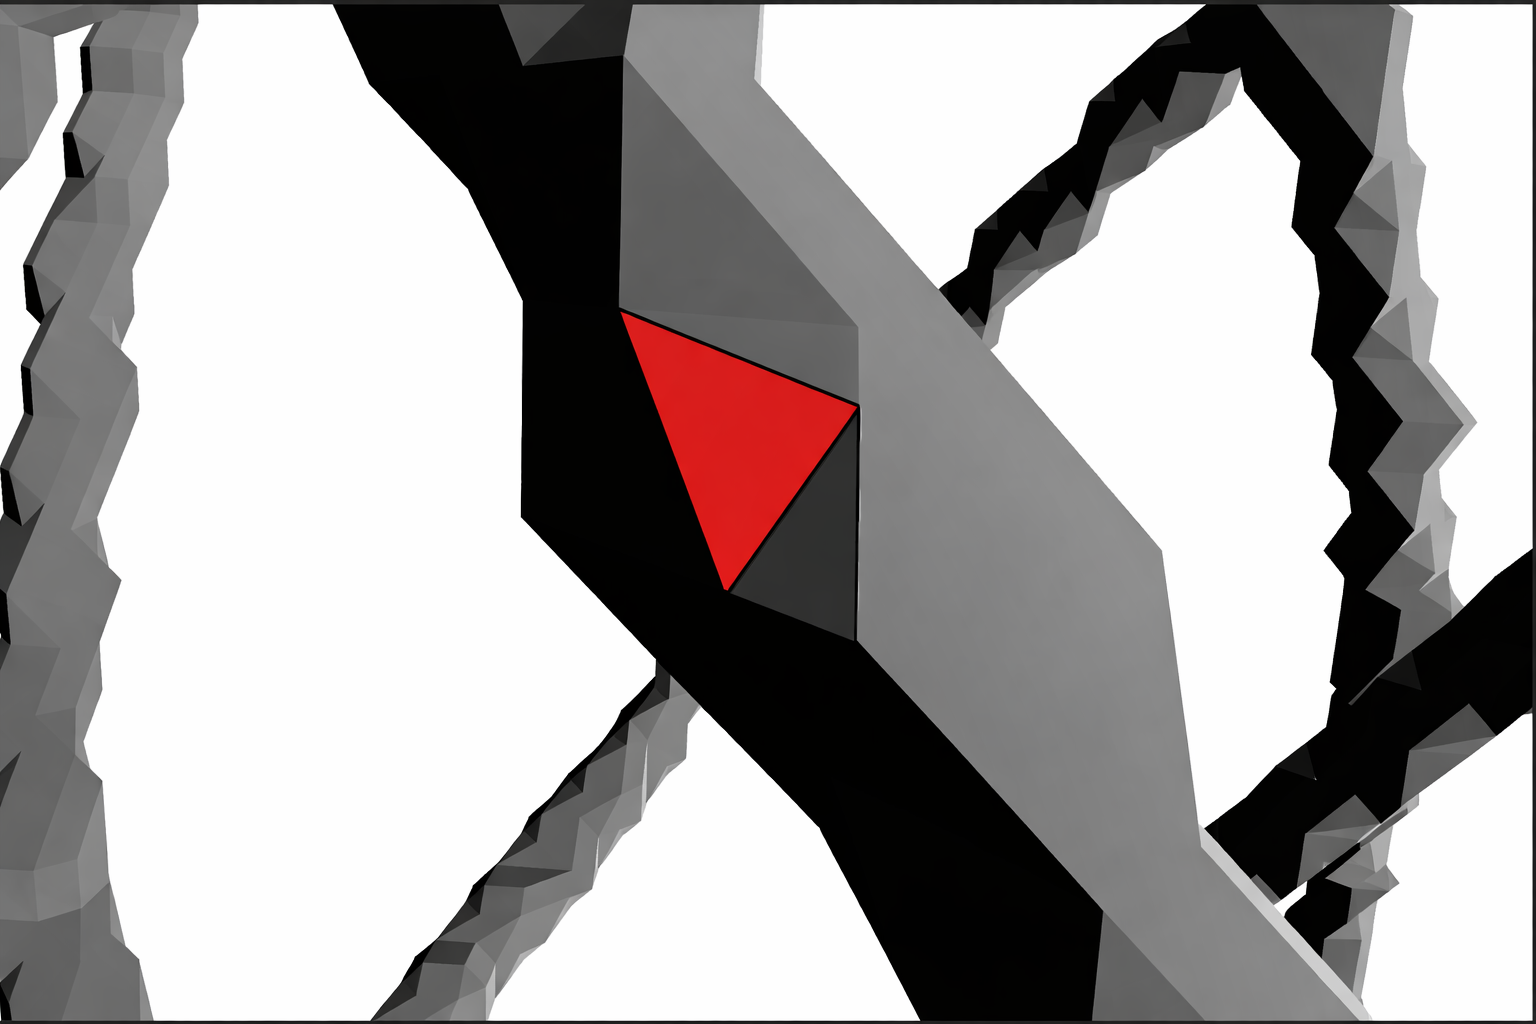
\includegraphics[width=0.62\textwidth]{img/cara.png}
    \caption{Identificación de una cara triangular en la malla asociada a una superficie triangulada. La región resaltada en rojo representa un $2$-símplice del complejo simplicial bidimensional inducido por la triangulación, mientras que sus lados corresponden a $1$-símplices y sus vértices a $0$-símplices. La colección de estas caras, junto con sus aristas y vértices, determina la estructura combinatoria de la superficie discretizada.}
    \label{fig:dos_simplice_cara}
\end{figure}

Desde un punto de vista topológico, esta construcción permite verificar si la malla define una $2$-variedad. En efecto, si cada arista pertenece exactamente a dos triángulos y el entorno de cada vértice es homeomorfo a un disco, entonces la realización geométrica del complejo es una superficie. Dado que la triangulación es finita, esta superficie es compacta; y si además no existen aristas de borde, se trata de una superficie cerrada.
En términos computacionales, aunque la construcción del grafo a partir del archivo STL captura correctamente la estructura de adyacencia entre vértices, es fundamental almacenar explícitamente las caras triangulares para preservar la naturaleza bidimensional del objeto. Esto se logra manteniendo un registro de las ternas de vértices que definen cada triángulo, lo cual permite reconstruir el complejo simplicial completo.
Finalmente, esta representación discreta resulta fundamental para el análisis mediante técnicas modernas de aprendizaje profundo sobre gráficas, como las Graph Neural Networks (GNNs), ya que facilita tanto la visualización —apoyada en herramientas como \textbf{matplotlib}— como el procesamiento estructural de los nudos desde una perspectiva combinatoria y geométrica.

\begin{figure}[H]
    \centering
    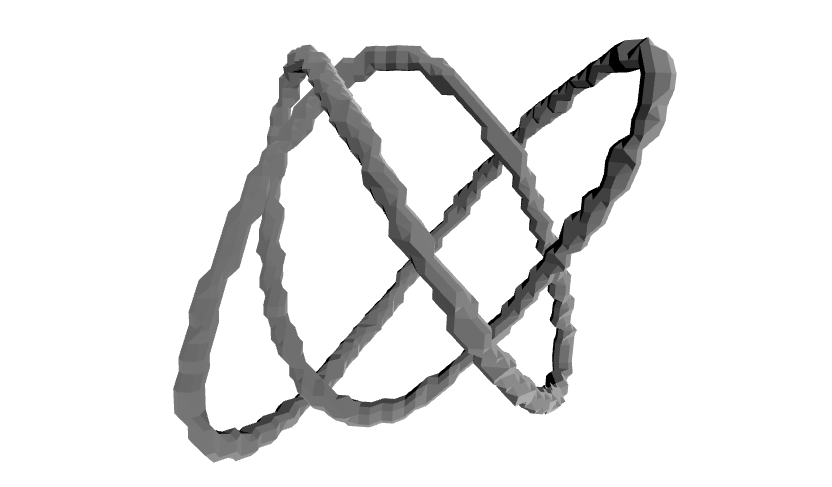
\includegraphics[width=0.62\textwidth]{img/superficie.png}
    \caption{Superficie triangulada generada a partir de una curva de Lissajous engrosada en $\mathbb{R}^3$. La discretización induce un complejo simplicial bidimensional $K=(V,E,F)$, en el cual cada cara corresponde a un $2$-símplice. La superficie es compacta y sin frontera, es decir, una superficie cerrada, y posee género $1$, por lo que es topológicamente equivalente a un toro. La representación presenta una estructura entrelazada con auto-intersecciones aparentes en su proyección, producto de la parametrización periódica subyacente. Esta modelación discreta permite el análisis de propiedades topológicas mediante su estructura combinatoria, incluyendo el cálculo de invariantes como la característica de Euler.}
    \label{fig:dos_simplice_superficie}
\end{figure}

\section{Muestreo por árbol generador mínimo}
Durante el análisis de la estructura de la gráfica, se identificó un problema asociado al procesamiento de los datos, derivado de las limitaciones del entorno local. Para abordar este desafío, se desarrolló un conjunto de métodos y técnicas orientadas a realizar un muestreo eficiente sobre la superficie y los nodos del grafo, preservando al mismo tiempo su estructura original.

Uno de los principales retos en la obtención de muestras de una gráfica consiste en definir un esquema de recorrido que evite imponer un orden arbitrario y garantice que cada nodo sea visitado a lo más una vez. Esta propiedad es fundamental para prevenir sesgos en los resultados, los cuales pueden surgir debido al orden en que los nodos son procesados.

Con el objetivo de realizar un muestreo aleatorio sin un orden predefinido, se proponen diversas técnicas que surgen de la integración de dos conceptos introducidos previamente en el Capítulo 2.

En primer lugar, se construye un árbol generador mínimo a partir de la matriz de adyacencia $A$ de la gráfica $G$, utilizando el algoritmo de Kruskal, el cual se describe a continuación:

\begin{algorithm}[H]
\caption{Algoritmo de Kruskal para el Árbol de Expansión Mínima (MST)}
\label{alg:kruskal}
\begin{algorithmic}[1]
\Require Grafo no dirigido \( G = (V, E) \) con pesos en las aristas
\Ensure Árbol de expansión mínima (MST)

\State \textbf{Inicializar} \( MST \gets \emptyset \) \Comment{Conjunto vacío para el MST}
\State \textbf{Ordenar} las aristas \( E \) en orden creciente de pesos
\State \textbf{Inicializar} estructura Union-Find para los vértices \( V \)

\For{cada arista \( (u, v) \in E \) en orden creciente de peso}
    \If{\textsc{Find}(u) \( \neq \) \textsc{Find}(v)} \Comment{Si u y v no están en el mismo componente}
        \State \( MST \gets MST \cup \{(u, v)\} \) \Comment{Añadir arista al MST}
        \State \textsc{Union}(u, v) \Comment{Unir los componentes de u y v}
    \EndIf
    \If{\textbf{Número de aristas en MST} \( = |V| - 1 \)} \Comment{MST completo}
        \State \textbf{break}
    \EndIf
\EndFor

\State \Return \( MST \) \Comment{Devolver el árbol de expansión mínima}
\end{algorithmic}
\end{algorithm}

Posteriormente a utilizar el algortimo de Kruskal para generar el árbol generador mínimo, convertimos el árbol resultante a una matriz simétrica de la siguiente forma : $A_{s} = A_{mst} + A_{mst}^T $.
El objetivo de generar el árbol generador mínimo es recorrer la estructura de la gráfica completa sin recorrer todas las aristas, sino sólo las más importantes que en este caso, son las que dan la estructura a la gráfica original.
Una vez obtenido el MST, procedemos a recorrerlo mediante un orden impuesto por el algoritmo "DFS", el cual es un algortimo que sirve para recorrer una gráfica en profundidad, es decir a lo "largo" asegurando así que visitaremos todos los nodos de dicha gráfica para preservar lo que nos interesa que es la estructura de la gráfica.
A continuación enunciaremos el algortimo DFS, y su implmentación en nuestro método:

\begin{algorithm}[H]
\caption{DFS Order}
\label{alg:DFS}
\begin{algorithmic}[1]
\Require Nodo actual $nodo$, lista de nodos visitados $visitados$, lista del orden $orden$
\Ensure Lista $orden$ con el orden en que los nodos son visitados
\Statex
\Function{DFS\_Order}{$nodo, visitados, orden$}
    \State $visitados[nodo] \gets \text{True}$
    \Comment{Marcar el nodo como visitado}
    \State Agregar $nodo$ a la lista $orden$
    \Comment{Registrar el nodo en el orden de visita}
    \ForAll{$vecino$ en posiciones donde $mst[nodo] = 1$}
        \If{$visitados[vecino] = \text{False}$}
            \State \Call{DFS\_Order}{$vecino, visitados, orden$}
            \Comment{Llamada recursiva para el vecino no visitado}
        \EndIf
    \EndFor
\EndFunction
\end{algorithmic}
\end{algorithm}

Posterior a establecer el orden en el que se recorrerá la gráfica, generamos un orden entre nodos para vistar los nodos más lejanos del nodo actual, asegurando de esta forma ir lo más lejos posible en el menor número de pasos.

\subsection{Muestreo por Esferas}
Una de las formas de mantener la estructura original de la gráfica es enfocándonos en su estructura local, es decir, podemos mirar a partir de un nodo  $v$ su vecindario, así como también tomar una pequeña esfera $S_v(r)$ con radio $r$ y centro en $v$ que interseque su vecindario $N_G(v)$, para así mantener las propiedades locales y poder asegurar que se preserve la estructura recibida.
\\ Para identificar la muestra resultado de la intersección entre $N_G(V)$ y la esfera $S_v(r)$ se ha construido un método denominado Método polar para desviaciones normales \cite[p.~122-123]{Knuth}.
A continuación describiremos un algortimo que sirve como base a la implementación realizada para muestrear uniformemente puntos en el volumen de una esfera, se conoce cómo \textit{Método polar para desviaciones normales} o \textit{Método polar de Marsaglia}.

\begin{algorithm}[H]
\caption{Método polar para desviaciones normales}
\label{alg:desviaciones}
\begin{algorithmic}[1]
\State \textbf{P1} [Obtener variables uniformes]
\State Generar dos variables aleatorias independientes \( U_1, U_2 \sim U(0,1) \).
\State Asignar \( V_1 \gets 2U_1 - 1 \), \( V_2 \gets 2U_2 - 1 \), ahora \( V_1, V_2 \sim U(-1,1) \).

\State \textbf{P2} [Calcular \( S \)]
\State Asignar \( S \gets V_1^2 + V_2^2 \).

\State \textbf{P3} [¿Es \( S \geq 1 \)?]
\If{\( S \geq 1 \)}
    \State Regresar al paso \textbf{P1}.
\EndIf

\State \textbf{P4} [Calcular \( X_1, X_2 \)]
\State Asignar:
\[
X_1 \gets V_1 \sqrt{\frac{-2 \ln S}{S}}, \quad X_2 \gets V_2 \sqrt{\frac{-2 \ln S}{S}}
\]

\end{algorithmic}
\end{algorithm}
Para probar la validez del método anterior utilizaremos geometría analítica y un poco de cálculo.
\begin{proof}
Notamos que si $S < 1 $ en el paso $P3$, el punto en el plano cartesiano con las coordenadas $(V_1,V_2)$ es un punto aleatorio uniformemente dsitribuido dentro del círculo unitario.
\\Transformando a coordenadas polares tenemos que:
$V_1 = Rcos\theta$, $V_2 = Rsen\theta$ y sustituyendo tenemos que:
\[
S = R^2, \hspace{5pt} X_1=(Rcos\theta) \sqrt{\frac{-2lnS}{R^2}}, \hspace{5pt} X_2=(Rsen\theta) \sqrt{\frac{-2lnS}{R^2}}
\]
De aquí observamos que:
\begin{align*} 
X_1 &= (Rcos\theta) \sqrt{\frac{-2lnS}{R^2}} \\ 
 &=  Rcos\theta \frac{\sqrt{-2lnS}}{\sqrt{R^2}}\\
 &= Rcos\theta \frac{\sqrt{-2lnS}}{|R|} \\
&= cos\theta \sqrt{-2lnS}
\end{align*}
Pues $R >0$
De igual forma $X_2 = sen\theta\sqrt{-2lnS}$.
Utilizando coordenadas polares y haciendo: 
\[
R' = \sqrt{-2lnS}, \hspace{1cm}\theta' = \theta
\]
Tenemos que $X_1 = R'cos\theta', \hspace{5pt} X_2 = R'sen\theta'$
Así, observamos que $R'$ y $\theta'$ son independientes pues $R$ y $\theta$ lo son.
También $\theta' \sim U(0,2\pi)$ pues es el rango de las funciones $sen$ y $cos$. 
\\A su vez notamos que:
\begin{align*}
P(R' \leq r) &=P(-2lnS \leq r^2)\\
&= P(S \geq e^{\frac{-r^2}{2}})
\end{align*}
Por otro lado , como $S \sim U(0,1)$ entonces su función de distribución accumulada es :
\[
F(s) = P(S\leq s) = s, \hspace{1cm} s \in[0,1]
\]
De esta forma la probabilidad complementaria es:
\begin{align*}
P(S < s) &= 1 - P(S \geq s)\\
P(S \geq s) &= 1 - P(S<s)
\end{align*}
Por tanto:
\begin{align*}
P(S\geq e^{\frac{-r^2}{2}} ) &= 1 -P(S < e^{\frac{-r^2}{2}})\\
&= 1 - e^{\frac{-r^2}{2}}  
\end{align*}

Ahora, la probabilidad que $R'$ esté entre $r$ y $r +dr$ es la derivada de $1-e^{\frac{-r^2}{2}}$ que es igual a $re^{\frac{-r^2}{2}}dr$. Similarmente la probabilidad de que $\theta'$ esté entre $\theta$ y $\theta + d\theta$ es $\frac{1}{2\pi}d\theta$
De esta forma, la probabilidad conjunta de $X_1 \leq x_1$ y $X_2 \leq x_2$ es:

\begin{align*}
    \int_{\{(r,\theta) | rcos\theta \leq x_1 , r sen\theta \leq x_"\}} \frac{1}{2\pi}e^{\frac{-r^2}{2}} r dr d\theta &= \frac{1}{2\pi} \int_{\{(x,y) | x \leq x_1, y \leq x_2\}}e^{\frac{-(x^2 + y^2)}{2}} dx dy \\
    &= \left(  \sqrt{\frac{1}{2\pi}} \int_{-\infty}^{x_1} e^{\frac{-x^2}{2}}dx\right)\left(  \sqrt{\frac{1}{2\pi}} \int_{-\infty}^{x_2} e^{\frac{-y^2}{2}}dy\right)
\end{align*}

Lo cual prueba que $X_1$ y $X_2$ son variables aleatorias independientes con distribución normal, tal como se requería.
    
\end{proof}
Basado en el algortimo 3, podemos derivar un método que permita generar puntos aleatorios dentro de una esfera en 3 dimensiones.
Sean $U_1,U_2 \sim \mathcal{U}(0,1)$ entonces, hacemos $V_1,V_2$ y $S$ como:
\[
    V_1 = 2U_1-1, \hspace{5pt} V_2=2U_2-1, \hspace{5pt} S = V_1^2+V_2^2
\]
Notamos entonces que $V_1,V_2 \sim \mathcal{U}(-1,1)$
\\Por otro lado, sabemos que la esfera $\mathbb{S}^2$ tiene las siguientes coordenadas:
\[
X = sen(\theta)cos(\phi),  \hspace{5pt} Y = sen(\theta)sen(\phi),  \hspace{5pt} Z = cos(\theta) 
\]

Notamos que $Z = cos(\theta)$ tiene un rango de valores de $[-1,1]$, entonces utilizando la transformación $Z = 2S-1$ para $S = V_1^2 + V_2^2 \leq 1$ esto implica que. $Z=cos(\theta) = 2S-1 \in [-1,1]$
Por otro lado;

\begin{align*}
    cos^2(\theta) + sen^2(\theta) &= 1\\
    sen^2(\theta)&=1-cos^2(\theta)\\
    sen^2(\theta)&=1-Z^2\\
    sen(\theta)&=\sqrt{1-Z^2}
\end{align*}

Por tanto:

\begin{align*} \tag{1} \label{XY}
  X = \sqrt{1-Z^2} cos(\phi), \hspace{1cm} Y=\sqrt{1-Z^2}sen(\phi)  
\end{align*}


Por otro lado, notamos que por construcción

\begin{align*}
S &= V_1^2 + V_2^2\\
\sqrt{S}  &= \sqrt{V_1^2 + V_2^2}
\end{align*}

Y además, en el plano $XY$

\begin{align*}
    cos(\phi) &= \frac{V_1}{\sqrt{V_1^2 + V_2^2}}\\
    &= \frac{V_1}{\sqrt{S}}
\end{align*}

Análogamente: $sen(\phi) = \frac{V_2}{\sqrt{S}}$


Sustituyendo en \ref{XY}

\begin{align*}
    X &= \sqrt{1-Z^2} \frac{V_1}{\sqrt{S}}\\
      &= \frac{\sqrt{1- Z^2}}{\sqrt{S}} V_1\\
      &= \sqrt{\frac{1-Z^2}{S}} V_1
\end{align*}

Desarrollando $\sqrt{\frac{1-Z^2}{S}}$ :

\begin{align*}
    \sqrt{\frac{1-Z^2}{S}} &= \sqrt{\frac{1 - (2S-1)^2}{S}}\\
    &= \sqrt{\frac{1-((2S)^2 + (4S)(-1)+1)}{S}}\\
    &= \sqrt{\frac{1 - (4S^2 -4S +1)}{S}}\\
    &= \sqrt{\frac{-4S^2 - 4S}{S}}\\
    &= \sqrt{\frac{4S(-S+1)}{S}}\\
    &= \sqrt{4(1-S)}\\
    &= \sqrt{4}\sqrt{1-S}\\
    &=2\sqrt{1-S} 
\end{align*}

Es decir se toma la parte positiva de la raiz cuadrada ya que se están normalizando coordenadas, por otro lado notamos que $1-S \geq 0$ pues $S \leq 1$.
Así, por convención hacemos $\alpha = 2\sqrt{1-S}$, por tanto
$X = \alpha V_1$ y análogamente,
$Y = \alpha V_2$
De esta forma la generación de puntos aleatorios en la superficie de la esfera es:
\[
(\alpha V_1, \alpha V_2, 2S-1)
\]
Donde:
\begin{align*}
    X^2 + Y^2 + Z^2 &= (\alpha V_1)^2 + (\alpha V_2)^2 + (2S-1)^2\\
    &= \alpha^2(V_1^2 + V_2^2) + (2S-1)^2\\
    &= S(2\sqrt{1-S})^2 + (2S-1)^2\\
    &= 4S(1-S)+ 4S^2 -4S + 1\\
    &= -4S^2 + 4S + 4S^2 - 4S + 1\\
    &= 1
\end{align*}

Por último, para generar puntos aleatorios, dentro del volumen de la esfera, basta con generar un radio aleatorio de la siguiente forma: 
Dado $ R = \mathcal{U}(0,1)^\frac{1}{3}$, los puntos distribuidos dentro de la esfera están dados por:
\[
R(\alpha V_1, \alpha V_2, 2S-1)
\]

De esta forma mostraremos el algoritmo resultante en la siguiente forma;
\begin{algorithm}[H]
\caption{Generar Puntos Uniformes en una Esfera}
\label{alg:generaPuntos}
\begin{algorithmic}[1]
\Require Coordenadas del centro $h, k, l$, número de puntos $num\_puntos$
\Ensure Matriz de puntos uniformemente distribuidos en la esfera
\Statex
\Function{GenerarPuntosUniformes}{$h, k, l, num\_puntos$}
    \State Inicializar una lista vacía $puntos$
    \For{$i \gets 1$ \textbf{to} $num\_puntos$}
        \Repeat
            \State Generar $V1, V2 \gets \textsc{Uniform}(-1, 1)$
            \State Calcular $S \gets V1^2 + V2^2$
        \Until{$S < 1$}
        \State Calcular $a \gets \sqrt{1 - S}$
        \State Calcular $x \gets a \cdot V1 + h$
        \State Calcular $y \gets a \cdot V2 + k$
        \State Calcular $z \gets 2 \cdot S - 1 + l$
        \State Generar $r \gets \textsc{Uniform}(0, 1)^{\frac{1}{3}}$
        \State Agregar $[r \cdot x, r \cdot y, r \cdot z]$ a la lista $puntos$
    \EndFor
    \State \Return Matriz convertida a partir de $puntos$
\EndFunction
\end{algorithmic}
\end{algorithm}

\subsection{Reasignación de Adyacencias para Preservar la Estructura}

En el punto anterior notamos que cuando se elimina un nodo contenido dentro de la esfera de muestreo, los vecinos de este nodo pierden cierta informaciòn estructural contenida en el nodo eliminado, para evitar esto y preservar la estructura lo màs parecida posible a la inicial hacemos una reasignaciòn de adyacencias.

Describiremos a continuaciòn el proceso para eliminar un nodo $v$ de $G$ y que sus vecinos mantengan la adyacencia entre ellos, es decir si dos nodos $u,w$ eran vecinos de $v$ entonces después de eliminar $v$, $u$ y $w$ pasaran a ser vecinos entre ellos.

\begin{definition}
    Sea $G$ una gráfica y $A$ su matriz de adyacencia, entonces definimos al elemento $(A)_{ij}$ como el elemento ij-ésimo de la matriz $A$, donde $i,j \in \{0,...,\nu_G -1\}$
\end{definition}

\begin{example}
Sea la matriz $A$ dada por :
\begin{center}
\begin{equation}
A(G) =
\begin{pmatrix}
0 & 1 & 0 & 0 & 0 & 0\\
1 & 0 & 1 & 0 & 0 & 1\\
0 & 1 & 0 & 1 & 0 & 1\\
0 & 0 & 1 & 0 & 1 & 0\\
0 & 0 & 0 & 1 & 0 & 1\\
0 & 1 & 1 & 0 & 1 & 0
\end{pmatrix}
\end{equation}
    
\end{center}
Entonces los elementos $(A)_{02},(A)_{23},(A)_{54}$ son iguales a :
\begin{align*}
    (A)_{02} &= 0 \\
    (A)_{23} &= 1\\
    (A)_{54} &= 1
\end{align*}

\end{example}

Dada esta definición podemos ahora establecer una operación que sirve como punto de partida para implementar un método de eliminación controlada para los nodos de la gráfica.
La siguiente definición implementará una operación entre los elementos de la matriz de adyacencia $A_n$ donde $n$ representa el paso antes de realizar la operación y por ende la matriz $A_{n+1}$ denota a la matriz de adyacencia $A$ después de la operación.

\begin{definition}[Eliminación del nodo k]
Sea $G$ una gráfica $A_n$ la matriz de adyacencia en el paso $n$, $A_{n+1}$ la matriz de adyacencia en el paso $n+1$, $k$ el nodo a eliminar y $N_G(k)$ el vecindario del nodo $k$.\\
Entonces definimos la función,
\[
\psi : (A_n)_{ij} \times (A_n)_{kj} \rightarrow (A_{n+1})_{ij}
\]
Dada por:
\begin{equation}
    \psi_{ij} := (A_{n+1})_{ij}= \left\{ \begin{array}{lcc} (A_n)_{ij} \hspace{5pt} +_{or} \hspace{5pt} (A_n)_{kj} & , & i \neq j, j \neq k \\ \\0 & , & k = j, i=j \\  \end{array} \right.
\end{equation}
Con $i \in N_G(k) \cup \{k\}$, además $\psi_{kj} = 0$, $\forall \hspace{5pt} j \in \{0,...,\nu_G\}$
    
\end{definition}

\begin{example}
    Dada la matriz $A_0 = A(G)$ del ejemplo (2), $k = 5$, $\nu_G = 6$, $j \in \{0,...5\}$ entonces calcularemos los valores de $\psi$.

    Observamos que $N_G(k) = \{1,2,4\}$, entonces:

    \begin{align*}
    \psi_{10} : = (A_1)_{10 } &= (A_0)_{10} \hspace{5pt} +_{or} \hspace{5pt} (A_0)_{50} \\
     &= 1 \hspace{5pt} +_{or} \hspace{5pt} 0 \\
     &= 1\\
    \psi_{11} := (A_1)_{11} &= 0 \\
    \psi_{12} := (A_1)_{12} &= (A_0)_{12}  \hspace{5pt} +_{or} \hspace{5pt} (A_0)_{52}\\
        &= 1 \hspace{5pt} +_{or} \hspace{5pt} 1\\
        &= 1\\
        \psi_{5j} := (A_1)_{5j} &= 0 \hspace{1cm} \forall \hspace{5pt} j \in \{0,...,5\}
    \end{align*}
    
    
    

    Y notamos que análogamente para $i = \{2,4\}$.
    De esta forma la matriz $A_1$ quedaría de la siguiente forma:

    \begin{center}
\begin{equation}
A_1(G) =
\begin{pmatrix}
0 & 1 & 0 & 0 & 0 & 0\\
1 & 0 & 1 & 0 & 1 & 0\\
0 & 1 & 0 & 1 & 1 & 0\\
0 & 0 & 1 & 0 & 1 & 0\\
0 & 1 & 1 & 1 & 0 & 0\\
0 & 0 & 0 & 0 & 0 & 0
\end{pmatrix}
\end{equation}
\end{center}
\end{example}
Así, hemos definido una operación para las matrices de adyacencia donde, dado un nodo $k$ podemos eliminarlo de dicha matriz, es decir, $(A)_{kj}$,$(A)_{ik} = 0$, donde $i,j \in \{0,...,\nu_G \}$ asegurando que sus vecinos preserven la adyacencia entre ellos, sin modificar la estructura original de la gráfica.
\\De esta forma podemos definimos el algoritmo de la siguiente manera:
\begin{algorithm}[H]
\caption{Eliminar Nodo con Redistribución de Adyacencias}
\label{alg:elimnaAdyacencias}
\begin{algorithmic}[1]
\Require Nodo a eliminar $nodo$, matriz de adyacencia $matrizAdj$
\Ensure Matriz de adyacencia actualizada sin el nodo y con conexiones redistribuidas
\Statex
\Function{EliminaNodoConAdyacencia}{$nodo, matrizAdj$}
    \State Obtener los vecinos del nodo: $neighbors \gets \textsc{Where}(matrizAdj[nodo] = 1)$
    \Comment{Lista de nodos directamente conectados a $nodo$.}
    \ForAll{$v$ en $neighbors$}
        \State $matrizAdj[v] \gets \textsc{LogicalOr}(matrizAdj[v], matrizAdj[nodo])$
        \Comment{Redistribuir conexiones del nodo eliminado a sus vecinos.}
    \EndFor
    \State $matrizAdj[nodo, :] \gets 0$
    \Comment{Eliminar todas las conexiones salientes del nodo.}
    \State $matrizAdj[:, nodo] \gets 0$
    \Comment{Eliminar todas las conexiones entrantes al nodo.}
    \State \Return $matrizAdj$
\EndFunction
\end{algorithmic}
\end{algorithm}

\subsection{Método general para la reducción de nodos}

Una vez establecidos los métodos descritos anteriormente, es posible combinar sus principios para desarrollar un enfoque generalizado de reducción de nodos. 
\\En esta sección, exploraremos en detalle dicho enfoque, examinando su complejidad computacional, describiendo su implementación paso a paso y destacando las ventajas clave que se derivan de su aplicación.

El proceso de muestreo eficiente en una gráfica se basa en reducir el número de nodos mientras se conservan sus propiedades clave. Primero, se genera un orden de recorrido utilizando un árbol generador mínimo y el algoritmo DFS, lo que permite recorrer toda la gráfica y establecer un orden basado en DFS.

En el ciclo principal, se iteran los nodos hasta alcanzar el tamaño deseado de la muestra. Se calculan las distancias promedio entre los nodos ordenados y el centroide de la muestra, priorizando los más lejanos para evitar sesgos. Con el nuevo orden, se generan puntos alrededor de cada nodo utilizando una esfera, identificando y eliminando vecinos dentro de un radio definido, manteniendo la adyacencia. Este proceso se repite hasta obtener la muestra requerida. El algoritmo se divide en fases para facilitar su comprensión. 
\begin{algorithm}[H]
\caption{Método General}
\label{alg:metodoGeneral}
\begin{algorithmic}[1]
\Require Lista de nodos con coordenadas $x$, Matriz de adyacencia $adjacency$, Tamaño de muestra $size$, Radio $alcance$, Tamaño de la muestra de esfera $esfera\_size$
\Ensure Nueva lista de nodos $new\_x$, Matriz de adyacencia Actualizada $new\_adj$
\Statex
\Function{Sampling}{$x, adjacency, size, alcance, esfera\_size$}
    \State Obtener el árbol generador mínimo (MST) desde $adjacency$ \Comment{Algoritmo \ref{alg:kruskal}}
    \State Inicializar $visited[] \gets FALSE$ ; $order[] \gets empty\_list$
    \State Obtener orden mediante DFS $dfs\_order(0, visited, order) $\Comment{Algoritmo \ref{alg:DFS}} 

    \State Inicializar $removed\_nodes[] \gets empty\_list$; $queue[] \gets copy(order)$
    
    \While{$number\_nodes - removed\_nodes \geq size$}
        \If{$removed\_nodes$ no es vacío}
            \State $dist \gets dist(currency\_node,centroid) $
            \State Ordena $queue$ por distancias en orden descendente
        \EndIf
        \State Obtener coordenadas del primer elemento de $queue$.
        \\ \hfil $idx \gets queue.pop()$; $h, k, l \gets x[idx]$ 
        \State Obtenemos esfera uniforme \Call{GeneraPuntosUniformes}{$idx$} \Comment{Algoritmo \ref{alg:generaPuntos}}
        \State Hacemos $neighbors \gets neighbors \cap GeneraPuntosUniformes(idx)$
        \ForAll{$vecinos \in vecinos - eliminados$}
            \State \Call{EliminaNodoConAdyacencia}{$n$,$adyacency$} \Comment{Algoritmo \ref{alg:elimnaAdyacencias}}
        \EndFor
    \EndWhile
    \State \Return $new\_x, new\_adj$
\EndFunction
\end{algorithmic}
\end{algorithm}
\subsection{Análisis de Complejidad}

El análisis de complejidad de nuestro algoritmo se realiza descomponiendo sus principales componentes y justificando cada cálculo. La construcción del Árbol Generador Mínimo (MST) utiliza el algoritmo de Kruskal, que tiene una complejidad de \( \mathcal{O}(E \log(V)) \)\cite{Introduction-toalgorithm}, donde \( E \) es el número de aristas y \( V \) el número de vértices de la gráfica. Este paso es esencial para establecer una estructura inicial que guía el muestreo de nodos.
El siguiente paso es ordenar los nodos del grafo mediante un recorrido en profundidad (DFS), cuya complejidad es \( \mathcal{O}(V + E) \)\cite{Introduction-toalgorithm}. Esto se debe a que el DFS visita cada vértice y cada arista exactamente una vez. Este orden nos permite recorrer sistemáticamente los nodos y controlar las operaciones de muestreo.

El bucle principal del algoritmo, que se ejecuta hasta alcanzar el tamaño deseado de la muestra, domina la mayor parte del costo computacional, en el peor de los casos este bucle se ejecuta \(V\) veces, considerando que el tamaño de la muestra puede representar una cota ya que en cada iteración se elimina un nodo por tanto su costo podría acotarse por \(\mathcal{O} (V)\). 

Dentro de este bucle, el cálculo de distancias entre los nodos y el centroide de la muestra se calcula mediante la norma euclideana, es decir se calcula la distancia a lo más $V$ veces y se repite por el número $d$ de dimensión que en este caso $d=3$ por tanto la complejidad total es: $\mathcal{O}(V)$ .

Luego, la complejidad del algoritmo para generar la muestra uniforme está determinado por el número de veces que se ejecuta su bucle principal, ya que, las operaciones realizadas no dependen del número de puntos a generer, por lo tanto la complejidad es constante, de esta forma el número de pasos que realiza el método es en el orde de $esfera\_size$ que, para términos de la implementación de dicho algorimot, siempre es constante.

La intersección de los vecinos generados en la esfera con los vecinos del nodo en la matriz de adyacencia tiene un costo lineal de \( \mathcal{O}(V) \). Este cálculo depende del tamaño de los conjuntos comparados, donde el conjunto mayor está determinado por el número de vértices de la gráfica. Una vez identificados los nodos dentro de la esfera, el algoritmo actualiza la matriz de adyacencia. Dado que esta matriz tiene un tamaño de \( V \times V \), las operaciones de reajuste tienen un costo de \( \mathcal{O}(V^2) \).

Finalmente, los nodos eliminados deben ser descartados de la matriz de adyacencia, lo que implica un costo adicional de \( \mathcal{O}(V) \) por le número de pasos k, donde \( k \) es el número de nodos eliminados que para terminos de la implementación lo podemos dejar como una constante, por lo tanto la complejidad final sería $\mathcal{O}(V)$.
 Este costo se suma al procesamiento necesario para mantener la consistencia de la estructura de datos.
Resumiendo , notamos que las operaciones más costosas que otorgan la complejidad final al algoritmo es la obtención del MST $\mathcal{O}(E\log V)$ y las iteraciones del bucle principal, que resulta ser $\mathcal{O}(V * V^2) = \mathcal{O}(V^3)$ pues, las operaciones se ejecutan $V$ veces multiplicado por el reordenamiento de la matriz de adyacencia, entonces dado las dos operaciones mas costosas en diferentes fases del algortimo la complejidad final está dada por: $\mathcal{O}(E \log V +  V^3)$. 
\\Como observación final, en el peor de los casos sabemos que $E = V^2$, pero como estamos trabajando con un tipo de gráficas especiales, para este caso $E \neq V^2$, en específico $E < V^2$


captura equivarianzas sobre la superficie por eso los resultados parecen ser mejores.